

\noindent In \exrange{exercise-4.4.1}{exercise-4.4.6}, determine whether a given function is a power function. If yes, identify the coefficient $k$ and the exponent $p$. If not, say so.

\begin{exercise}\label{exercise-4.4.1}
$\displaystyle y= \frac{\sqrt{x^3}}{0.1x}$
\end{exercise}

\begin{solution}
$y=10x^{1/2}$; $k=10$; $p=\frac{1}{2}$
\end{solution}


\begin{exercise}
$\displaystyle y= \frac{\sqrt{0.01x^3}}{\sqrt{x}}$
\end{exercise}

\begin{solution}
$y=0.1x$; $k=0.1$; $p=1$
\end{solution}


\begin{exercise}
$\displaystyle g(x)=\frac{x^{\frac{5}{3}}}{4x^{\frac{1}{4}}}$
\end{exercise}

\begin{solution}
$y=\frac{1}{4}x^{17/12}$; $k=\frac{1}{4}$; $p=\frac{17}{12}$
\end{solution}


\begin{exercise}
$\displaystyle h(x)=2x^{\frac{3}{2}}-x^{-2}$
\end{exercise}

\begin{solution}
Not a power function.
\end{solution}


\begin{exercise}
$\displaystyle y=\sqrt{\frac{x^5}{9x}}$
\end{exercise}

\begin{solution}
$y=\frac{1}{3}x^2$; $k=\frac{1}{3}$; $p=2$
\end{solution}


\begin{exercise}\label{exercise-4.4.6}
$\displaystyle f(x)=(\sqrt{2^x})^2$
\end{exercise}

\begin{solution}
Not a power function.
\end{solution}







\begin{exercise}
Four power functions $y=kx^p$ are graphed below, where $p$ is a negative integer. In each of the graphs, is the exponent $p$ even or odd? Is the coefficient $k$ positive or negative?

\noindent
\begin{tabular}{cccc}
\begin{tikzpicture}[scale=0.5]
\begin{axis}[grid=none,
xmin=-3,xmax=3,
ymin=-3,ymax=3,
xtick=\empty,
ytick=\empty,
minor tick={},
xlabel={}, ylabel={},
]
\addplot[domain=-2.5:-0.1] {1/x};
\addplot[domain=0.1:2.5] {1/x};
\end{axis}
\end{tikzpicture}
&
\begin{tikzpicture}[scale=0.5]
\begin{axis}[grid=none,
xmin=-3,xmax=3,
ymin=-3,ymax=3,
xtick=\empty,
ytick=\empty,
minor tick={},
xlabel={}, ylabel={},
]
\addplot[domain=-3:-0.5] {-1/x^2};
\addplot[domain=0.5:3] {-1/x^2};
\end{axis}
\end{tikzpicture}
&
\begin{tikzpicture}[scale=0.5]
\begin{axis}[grid=none,
xmin=-3,xmax=3,
ymin=-3,ymax=3,
xtick=\empty,
ytick=\empty,
minor tick={},
xlabel={}, ylabel={},
]
\addplot[domain=-2.5:-0.1] {-1/x};
\addplot[domain=0.1:2.5] {-1/x};
\end{axis}
\end{tikzpicture}
&
\begin{tikzpicture}[scale=0.5]
\begin{axis}[grid=none,
xmin=-3,xmax=3,
ymin=-3,ymax=3,
xtick=\empty,
ytick=\empty,
minor tick={},
xlabel={}, ylabel={},
]
\addplot[domain=-3:-0.5] {1/x^2};
\addplot[domain=0.5:3] {1/x^2};
\end{axis}
\end{tikzpicture} \\
(a) & (b) & (c) & (d)
\end{tabular}
\end{exercise}

\begin{solution}
(a) $p$ is odd; $k$ is positive.
(b) $p$ is even; $k$ is negative.
(c) $p$ is odd; $k$ is negative.
(d) $p$ is even; $k$ is positive.
\end{solution}


\begin{exercise}
Which of the following is a graph of $f(x)=-2x^{-5}$?

\begin{tabular}{ccc}
\begin{tikzpicture}[scale=0.5]
\begin{axis}[grid=none,
xmin=-3,xmax=3,
ymin=-3,ymax=3,
xtick=\empty,
ytick=\empty,
minor tick={},
xlabel={}, ylabel={},
]
\addplot[domain=-3:-0.5] {-1/x^2};
\addplot[domain=0.5:3] {-1/x^2};
\end{axis}
\end{tikzpicture}
&
\begin{tikzpicture}[scale=0.5]
\begin{axis}[grid=none,
xmin=-3,xmax=3,
ymin=-3,ymax=3,
xtick=\empty,
ytick=\empty,
minor tick={},
xlabel={}, ylabel={},
]
\addplot[domain=-3:-0.5] {1/x^2};
\addplot[domain=0.5:3] {1/x^2};
\end{axis}
\end{tikzpicture}
&
\begin{tikzpicture}[scale=0.5]
\begin{axis}[grid=none,
xmin=-3,xmax=3,
ymin=-3,ymax=3,
xtick=\empty,
ytick=\empty,
minor tick={},
xlabel={}, ylabel={},
]
\addplot[domain=-2.5:-0.1] {-1/x};
\addplot[domain=0.1:2.5] {-1/x};
\end{axis}
\end{tikzpicture} \\
(a) & (b) & (c)
\end{tabular}

\end{exercise}

\begin{solution}
(c)
\end{solution}


\begin{exercise}
Which of the following is a graph of $f(x)=2x^{-4}$?

\begin{tabular}{ccc}
\begin{tikzpicture}[scale=0.5]
\begin{axis}[grid=none,
xmin=-3,xmax=3,
ymin=-3,ymax=3,
xtick=\empty,
ytick=\empty,
minor tick={},
xlabel={}, ylabel={},
]
\addplot[domain=-3:-0.5] {1/x^2};
\addplot[domain=0.5:3] {1/x^2};
\end{axis}
\end{tikzpicture}
&
\begin{tikzpicture}[scale=0.5]
\begin{axis}[grid=none,
xmin=-3,xmax=3,
ymin=-3,ymax=3,
xtick=\empty,
ytick=\empty,
minor tick={},
xlabel={}, ylabel={},
]
\addplot[domain=-3:3] {x^2};
\end{axis}
\end{tikzpicture}
&
\begin{tikzpicture}[scale=0.5]
\begin{axis}[grid=none,
xmin=-3,xmax=3,
ymin=-3,ymax=3,
xtick=\empty,
ytick=\empty,
minor tick={},
xlabel={}, ylabel={},
]
\addplot[domain=-2.5:-0.1] {1/x};
\addplot[domain=0.1:2.5] {1/x};
\end{axis}
\end{tikzpicture} \\
(a) & (b) & (c)
\end{tabular}

\end{exercise}

\begin{solution}
(a)
\end{solution}



\begin{exercise}
Below you see graphs of the functions $\displaystyle y=x^{\frac{1}{2}}$,   $\displaystyle y=2x^{\frac{1}{2}}$, and $\displaystyle y=-x^{\frac{1}{2}}$. Decide which is which.

\begin{center}
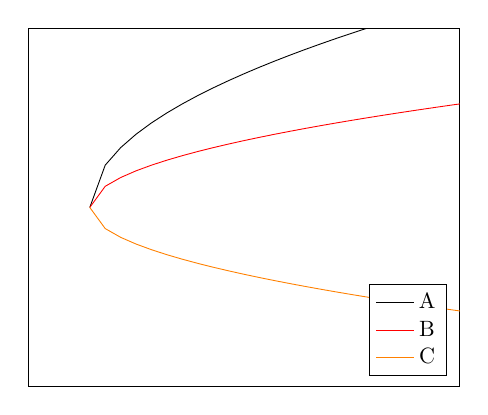
\begin{tikzpicture}[scale=0.8]
\begin{axis}[grid=none,
xmin=-0.5,xmax=3,
ymin=-3,ymax=3,
legend pos = south east,
xtick=\empty,
ytick=\empty,
minor tick={},
xlabel={}, ylabel={},
]
\addplot[domain=0:3] {2*sqrt(x)};
\addlegendentry{A}
\addplot[domain=0:3,red] {sqrt(x)};
\addlegendentry{B}
\addplot[domain=0:3,orange] {-sqrt(x)};
\addlegendentry{C}
\end{axis}
\end{tikzpicture}
\end{center}
\end{exercise}

\begin{solution}
Graph A is $y=2 x^{1/2}$, graph B is $y=x^{1/2}$, and graph C is $y=-x^{1/2}$.
\end{solution}


\begin{exercise}
Find a formula for a power function $f(x)=kx^p$ given numerically by:

\begin{center}
\begin{tabular}{|c|c|c|c|c|c|} \hline
$x$ & $0$ & $1$ & $2$ & $3$ & $5$ \\\hline
$f(x)$ & $0$ & $3$ & $3\sqrt{2}$ & $3\sqrt{3}$ & $3\sqrt{5}$ \\\hline
\end{tabular}
\end{center}
\end{exercise}

\begin{solution}
$f(x)=3x^\frac{1}{2}$
\end{solution}


\begin{exercise}
Find a formula for a power function $g(x)=kx^p$ given numerically by: 

\begin{center}
\begin{tabular}{|c|c|c|c|c|c|} \hline
$x$  & $0$ & $1$ & $2$ & $3$ & $5$ \\\hline
$g(x)$ & undefined & $2$ & $1$ & $\frac{2}{3}$ & $\frac{2}{5}$ \\\hline
\end{tabular}
\end{center}
\end{exercise}

\begin{solution}
$g(x)=2x^{-1}$
\end{solution}


\begin{exercise}
Consider a pendulum depicted below\footnote{Modified from a public domain image at https://en.wikipedia.org/wiki/Pendulum, accessed: 7/8/20}:

\begin{center}

\includegraphics[scale=0.2]{exercise-4.4-pendulum.png}
\end{center}

When the pendulum is displaced sideways from its resting position---called the equilibrium position---the force due to gravity will cause the pendulum to oscillate back and forth about the equilibrium position. The time, $T$, needed to execute one full cycle---a left swing and the right swing---is called the pendulum's period. The period $T$ depends on the length $L$ of the pendulum\footnote{https://en.wikipedia.org/wiki/Pendulum, accessed: 7/8/20} and the local acceleration due to gravity $g$:
\[
T=2\pi\sqrt{\frac{L}{g}}
.\]

\begin{parts}
\item With $g$ fixed, is $T$ a power function of $L$? In other words, is $T=kL^p$? If yes, find the coefficient and the exponent.


\item On the surface of the Earth, the acceleration due to gravity, $g$, is equal to $9.81\text{ m}/\text{sec}^2$ where $m$ stands for meters. Calculate the period of a pendulum of length $0.5 \text{ m}$ that happily oscillates in Kingston, RI.

\item An astronaut is standing on the surface of a faraway asteroid wondering about the acceleration due to gravity on the asteroid. The astronaut has a watch and a pendulum whose length is $0.3 \text{ m}$. The astronaut measures the period of the pendulum which turns out to be $5$ seconds. What is the acceleration due to gravity on the asteroid?
\end{parts}
\end{exercise}

\begin{solution}
\begin{parts}
\item yes; $T=\dfrac{2\pi}{\sqrt{g}}L^\frac{1}{2}$ where the coefficient is $\dfrac{2\pi}{\sqrt{g}}$ and the exponent is $\frac{1}{2}$.
\item approximately $1.42$ seconds.
\item approximately $0.47 \text{ m}/\text{sec}^2$.
\end{parts}

\end{solution}